\section{Introduction}

\subsection{Color gamuts}
There are several issues involved in reproducing colors from one device on another.
One important of these is the range of colors an imaging device, such as a camera, printer or monitor, is able to capture or provide.
Take for example an outdoor scene captured with a digital camera.
The camera will have a limited range of colors it can capture, so it can't capture the exact look of the real scene.
If someone then wants to display the image on a monitor, that monitor will have a limited range of colors that it can provide, so it might not be able to reproduce the same look as the camera captured.
This range of a set of colors that a device can reproduce is the color gamut~\cite{GamutMapping,HandbookGamutMapping}.

Since the colors can be represented in a three-dimensional space, the color gamut can as well.
This means that a color gamut has a volume and a surface, meaning that it is a three-dimensional polygon mesh.
This surface, which is \say{determined by a color gamut's extremities}~\cite{ColourImageScience}, is what is referred to as the gamut boundary, which is described by a gamut boundary descriptor (GBD)~\cite{HandbookGamutMapping}.

\subsection{Visualization of gamut boundaries}
\label{sec:intro-gbd-viz}
Because of the issues with color gamut and color gamut mapping, the need for visualizing the color gamut appeared~\cite{InteractiveGamutMapping}.
Visualizing color gamuts would allow people a better understanding of the gamuts and issues involved.
By visually displaying a color gamut, a human can intuitively see which color areas are outside or inside the gamut boundaries.
Even more intuitevely a person can compare two color gamuts visually and determine which colors of one gamut is outside another.
This can help understanding why an image doesn't appear right on a device and what needs to be done to map from one gamut to another in a pleasing or correct way.

There are multiple ways of visualizing a gamut, in both two and three-dimensional spaces~\cite{ColourImaging,InteractiveGamutMapping}.
Because colors can be represented in a three-dimensional space, three-dimensional visualizations properly represent the color gamut.
Two-dimensional gamuts have to remove one dimension or simplify the problem in another way~\cite{InteractiveGamutMapping}.

\subsection{Gamut boundary encoding in iccMAX}
The International Color Consortium (ICC) have created a standard specification for image technology color management which includes an architecture, profile format and datastructure~\cite{ColorManagement}.
The profile format allows manufactureres to create standard conforming profiles that define input or output color transformations~\cite{ColorManagement}.
There are several versions of the ICC specificatio, with iccMAX being the 5th and latest version.~\cite{IccMax}
The specification of iccMAX is currently in preliminary form, available for the public.
It introduces many improvements, like flexible illuminant and color matching function and a new GBD.
This new GBD is what this project aims to visualize.

As specified by the specification, an iccMAX Profile can have five different GBD tags, all of which are of the same tag type: gamutBoundaryDescriptionType (gbd)~\cite{IccMaxSpec}.
These tags have the signatures gbd0, gbd1, gbd2 and gbd3.
Each of the tags describe GBD's for different types of transforms.
gbd0 is \say{the gamut boundary of the reference medium gamut that was used for the creation of the perceptual transform}~\cite{IccMaxSpec}.
gbd1 is for the relative colorimetric transform, gbd2 is for the saturation intent transform and gbd3 is for the absolute colorimetric transform.

The gbd tag is described by a list of vertices and a list of faces.
Each vertex is a point in CIELAB color space that lay on the surface of the gamut boundary.
Each face is a geometric triangle comprised of three indices into the list of vertices.
All faces will together form a polygon mesh enclosing the gamut~\cite{BaselineGamut}.

According to the preliminary specification, the GBD is always described with PCS cordinates, but it optionally supports device coordinates with its own vertices and faces as well.
The number of PCS components, which must be 3 or more, is also specified in the tag.
When the gamut is viewed from the outside, the vertex order for each face is clockwise~\cite{IccMaxSpec}.

\subsection{Cross-platform and open source}
\label{sec:crossplatform-open}
One of the goals of this project is to only rely on open source projects, preferably with noncopylefted licenses~\cite{GnuFreeCategories}.
In addition, the project itself will be released as noncopylefted open source software licensed under the MIT license~\cite{MitLicense}.
There are many benefits of using and publishing open source software.
Most importantly the software can be used by everyone without worrying about licensing restrictions.
But open source also makes the software easier to maintain, inspires derivations and extensions.

In addition, this project will be built for cross-platform usage.
It is a fact today that many different platforms are used, from PC platforms such as Windows, Mac OS X and Linux, to mobile platforms such as Android and iPhone/iPad.
It is important that the software is available on all of these platforms so that as few users as possible are left out.
An additional requirement is that the software should without much effort work on new emerging platforms for a lonig-lasting life.

\subsection{Delimitation and assumptions}
The gbd tag in the iccMAX specification is flexible in that it supports 3 or more PCS coordinates and device values as well as PCS values.
This project will not concern itself with device values and will completely ignore their existence.
As they are optional, this will not be a problem.
Only 3 PCS channels and only the CIELAB PCS space will be supported.
Only the gbd0 tag will be visualized.

It is assumed that the preliminary specification is correct, and it will be followed to the point except for one case.
The preliminary specification specifies the gbd0, gbd1, gbd2 and gbd3 tags as gdb0, gdb1, gdb2 and gdb3 respectively.
It is assumed that this is wrong and that they will be corrected in the final version of the specification.

\section{Implementation}

\subsection{Platform and technologies}
To meet the requirements in Section~\ref{sec:crossplatform-open}, proper platform and technologies to build the application on have to be selected.
There are several good platforms available to use today.
One alternative is to write a native desktop application using cross-platform GUI toolkits, but this would mean compiling one version for each of the supported platforms, which will result in extra overhead.
Another alternative is using a virtualized platform such as Java, but Java is not supported on all platforms (e.g.\ iPhone/iPad).
While there are more alternatives, they have mostly the same limitatations.
What remains then is the web platform.
It is an open platform, it is supported by all major operating systems with a proper GUI interface, it supports hardware accelerated graphics, and the same source code will work on all browsers.
One might think that it would require an active internet connection, but in fact a website can work offline as well.
It can even be wrapped in another application including an internal web browser.
Thus the open web platform was selected as the base for building the application.

To allow faster development, while still having an appealing interface, the Boostrap library was used~\cite{Bootstrap}.
To make the application dynamic and reactive the AngularJS library was used~\cite{Angular}.
Both of these conform to web standards and work on many different browsers and versions.
To allow for easier builds, which helps user and developer adoption, the freely available Grunt build system together with npm as a dependency installer was used~\cite{Grunt,Npm}.

\subsection{iccMAX Profile GBD tag parsing}
The application consists of two major parts: GBD parsing and GBD visalization.
Since ICC Profiles use a binary format, a binary profile parser was written.
It is based on the preliminary specification of iccMAX, so any iccMAX Profile will be parsed correctly as long as the specification do not change.
The application searches through the Profile tag list until it finds the gbd0 tag.
The implementation can easily be extended to also parse the other GBD tags.
The GBD tag type is specified precisely in the specification, and the implementation follows this to the point.
Finally, the GBD tag data required to visualize the gamut (faces and PCS vertices) plus the PCS space is stored in a JavaScript structure to later be parsed by the visualizer.

\subsection{GBD visualization}
With the GBD data now parsed, the second major part, GBD visualization, can take place.
As discussed in Section~\ref{sec:intro-gbd-viz}, there exists several methods of visualizing gamut.
Since most consumer computers can now handle 3D graphics well, the development platform supports 3D hardware acceleration, and colors can be directly mapped in a 3D space, a CIELAB space 3D visualization was selected for the first implementation.
Other visualizations can be added at a later time.

To fully utilize 3D hardware rendering, WebGL was used~\cite{WebGl}.
But raw WebGL code is not easy nor fast to write, so a third party library called three.js was picked to handle the WebGL 3D rendering~\cite{ThreeJs}.
A three.js scene with an orthographics camera and CIELAB L*, a* and b* axes has been created.
The scene backround color is set to a grey color so that none of the colors at the gamut boundary are hidden.
It has no light sources, except one perfect white (255,255,255) ambient light that will make the model reflect its exact surface color.

To easier extend the application to create different visualizations, the simple concept of Model Makers was created.
A Model Maker is a structure which defines functions for making and destroying a 3D model from the gamut data.
There are currently three implemented Model Makers: Point Model Maker, Solid Model Maker and Wireframe Model Maker.
They are all extending the basic Model Maker to create point, solid and wireframe models respectively.
This system allows for switching between visualizations and extending with different visualizations at a later time.

The vertex coordinates of the boundary surface are converted to the WebGL rendering space from CIELAB.
This conversion involves setting L* as the y-axis, a* as the x-axis, b* as the inverse z-axis.
The b* has to be inversed because the z-axis of the rendering space points out of the screen.

To show the colors on the boundary surface, they have to be converted from CIELAB to an RGB format as this is the only format that WebGL supports.
Since sRGB is the default color profile in most web browsers, the colors are converted to this colorspace.
To accomplish this, the Chromatist JavaScript Library is used~\cite{Chromatist}.
This library support converting to and from XYZ to various other color spaces, such as sRGB and CIELAB.
To get to sRGB, the CIELAB data is first converted to XYZ using chromatist.cielab.Converter with D50 as the white point.
To get from XYZ to sRGB, chromatist.rgb.Converter is used with the default settings (sRGB, D65).
Since chromatist.rgb.Converter assumes that the XYZ whitepoint of the input values is the same as the RGB space settings (D65), the XYZ values are first chromatically adapted to D65 using chromatist.cat.Converter with the linear bradford algorithm.
The RGB values are finally clamped to the range [0,1] to avoid errors if the values are out of gamut.
For the solid and wrire frame models, the colors are linearly interpolated between the vertices of a face.

\section{Results}
The final working application can bee seen in Figure~\ref{fig:application}.
In this figure, a test profile has been loaded and is rendered as a solid model.
If no profile is loaded, only the three axes will be displayed.
To load a profile, a user can click the \say{Choose File} button or drag a profile from a file manager and drop it into the visualization box.
By default the application shows the solid rendered model, but by using the radio buttons to select between Solid, Wireframe and Point, a user can choose which rendering type to use.
The different types can be seen in Figure~\ref{fig:types}.

\begin{figure}[H]
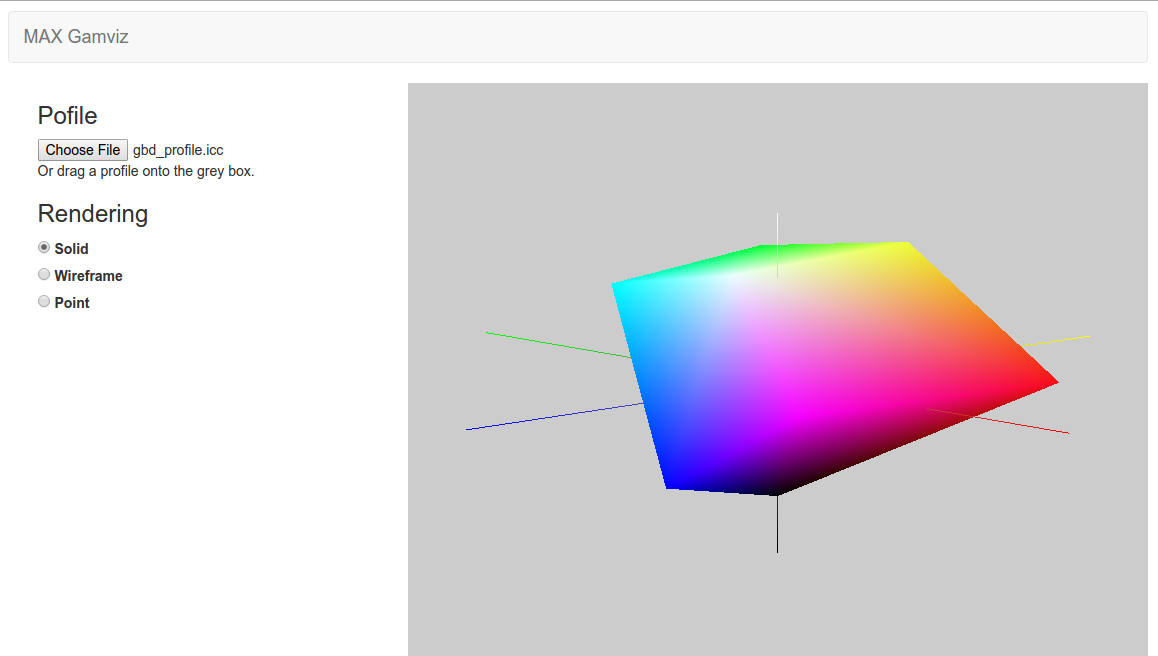
\includegraphics[width=\textwidth]{img/max-gamviz}
\caption{Running application with sRGB gamut example profile loaded as a solid model}
\label{fig:application}
\end{figure}

\begin{figure}[H]
	\centering
	\begin{subfigure}[t]{0.5\textwidth}
		\centering
		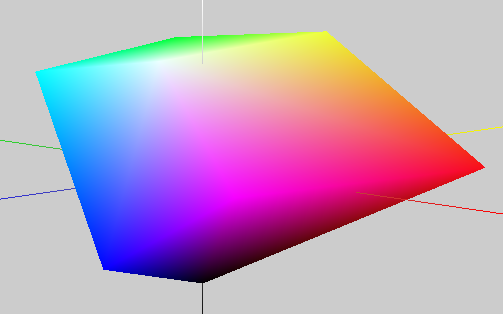
\includegraphics[width=0.9\textwidth]{img/solid}
		\caption{sRGB solid rendered GBD}
	\end{subfigure}%
	~
	\begin{subfigure}[t]{0.5\textwidth}
		\centering
		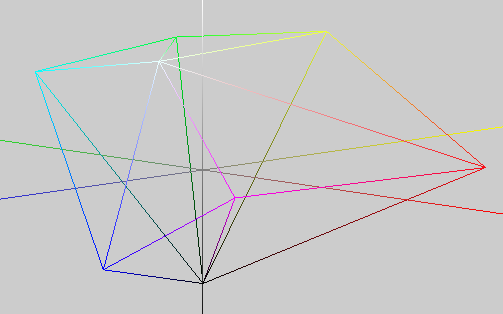
\includegraphics[width=0.9\textwidth]{img/wire}
		\caption{sRGB wireframe rendered GBD}
	\end{subfigure}%

	\begin{subfigure}[t]{0.5\textwidth}
		\centering
		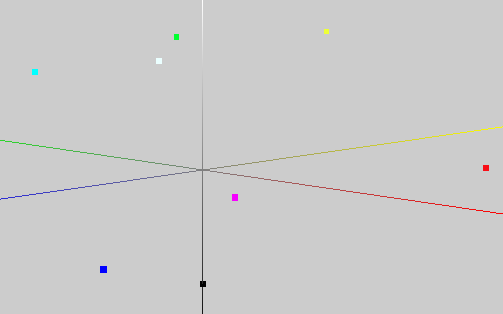
\includegraphics[width=0.9\textwidth]{img/points}
		\caption{sRGB point rendered GBD}
	\end{subfigure}
	\caption{Example sRGB GBD rendered as solid, wireframe and points}
	\label{fig:types}
\end{figure}

The application does not handle errors.
Loading a non-iccMAX Profile or a file which isn't an ICC Profile at all will silently fail without causing any issues in the application.

A user can move the camera by holding the left mouse button and moving the mouse.
This allows them to interactively inspect all angles of the gamut.
Figure~\ref{fig:sides} shows screenshots taken from different angles.

\begin{figure}[H]
	\centering
	\begin{subfigure}[t]{0.3\textwidth}
		\centering
		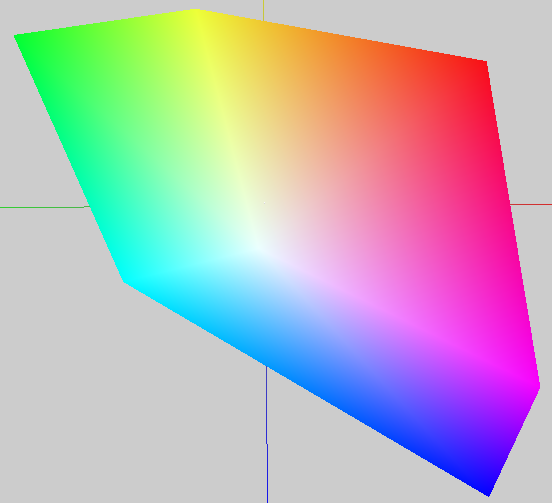
\includegraphics[width=0.9\textwidth]{img/solid-top}
		\caption{From top}
	\end{subfigure}%
	~
	\begin{subfigure}[t]{0.3\textwidth}
		\centering
		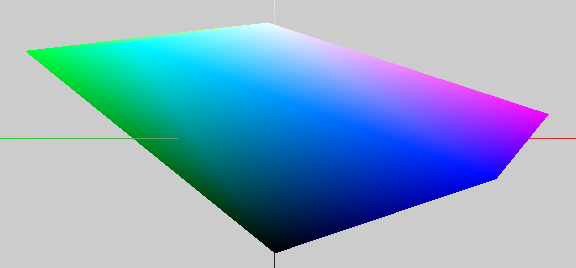
\includegraphics[width=0.9\textwidth]{img/solid-front}
		\caption{From front}
	\end{subfigure}%
	~
	\begin{subfigure}[t]{0.3\textwidth}
		\centering
		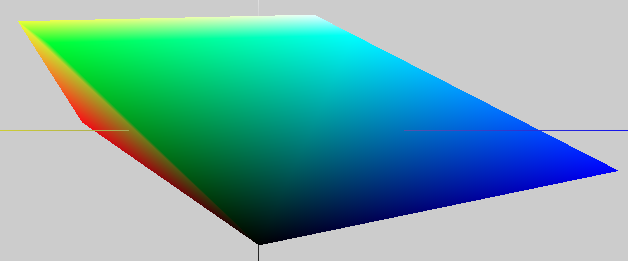
\includegraphics[width=0.9\textwidth]{img/solid-left}
		\caption{From left}
	\end{subfigure}%

	\begin{subfigure}[t]{0.3\textwidth}
		\centering
		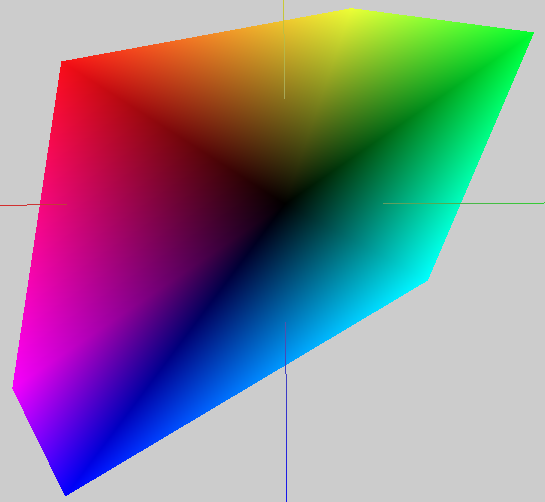
\includegraphics[width=0.9\textwidth]{img/solid-bottom}
		\caption{From bottom}
	\end{subfigure}%
	~
	\begin{subfigure}[t]{0.3\textwidth}
		\centering
		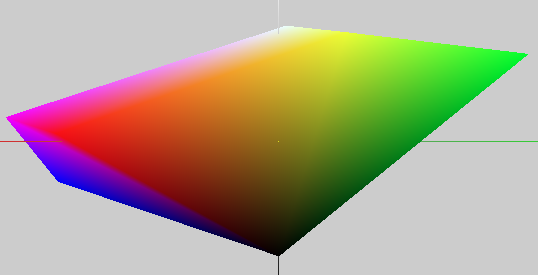
\includegraphics[width=0.9\textwidth]{img/solid-back}
		\caption{From behind}
	\end{subfigure}%
	~
	\begin{subfigure}[t]{0.3\textwidth}
		\centering
		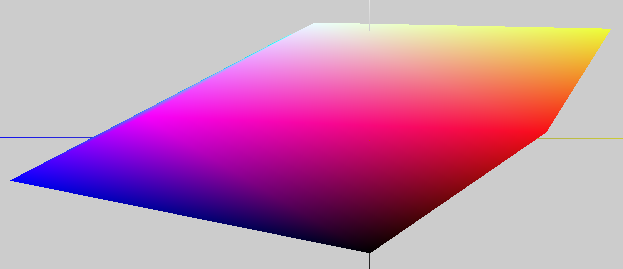
\includegraphics[width=0.9\textwidth]{img/solid-right}
		\caption{From right}
	\end{subfigure}
	\caption{Example sRGB GBD shown from different angles}
	\label{fig:sides}
\end{figure}

\section{Evaluation}
\subsection{User Interface}
The application has a very simple user interface, whith only a few options.
This makes it easier for a user to learn how to use the tool.
What the user interface is currently missing is proper error reporting and touch screen support.
Users should be presented with a warning message when a file can not be parsed.
To be truly cross-platform, the application needs to support touch devices.
While the current implementation does work on touch devices (e.g.\ smart phones), it does not support moving the camera with touch.
The visualization does also not properly scale to the screen size, causing the model to look stretched.
Both of these issues are not a limitation of the platform or technology, but with the available time for development.

\subsection{Correctness}
Since the GBD specified in the iccMAX Profile is in CIELAB space, the vertices shown will always be correct as long as the gamut specified is correct.
This can't be shown in the current application since the axes aren't numbered.
The displayed colors are limited by the sRGB gamut, so displaying a profile which has vertices outside the sRGB gamut will have their colors clamped and thus not displayed correctly.

\subsection{iccMAX parsing}
Implementing the iccMAX Profile parser was easier than expected.
The preliminary iccMAX specification is very clear and precise.
It is relatively easy to understand for a software developer, which is important as it will reduce the number of wrong implementations, make the behaviour concise over multiple systems and not hinder vendors to implement the specification.
The preliminary iccMAX specification has some errors, but this is expected and the final version should have these fixed.

\subsection{Fututre Work}
The application can be extended with many options.
Especially the rendering is of interest here, which is why the Model Maker system was created.
As shown by the implementation, creating multiple renderers is an easy job with Model Makers and the powerful three.js JavaScript library.
More fine grained control, like adjusting the background color is possible to add.

Currently the implementation on supports displaying the GBD with colors in sRGB space.
An addition to the application could be to let the users configure the color space and illuminant to use for the output colors.
It could even be possible to let the users upload an ICC Profile (not necessarily iccMAX) to use for the output color transformations.

\section{Conclusion}
The result clearly shows that it is possible and feasable to create an effective cross-platform open source application to visualize the GBD of iccMAX Profiles.
The tools and technology freely available makes this job easier than ever before.
And with the clear and precise specification of iccMAX, writing a binary parser is not a problem.
